\section{Conjugated segments and rigid fragments}

Conjugated segments are described in a separate \xml file. An example for \dcvt is shown in listing~\ref{list:conjugated_segments}.



\clearpage
\begin{figure}[ht]
\centering
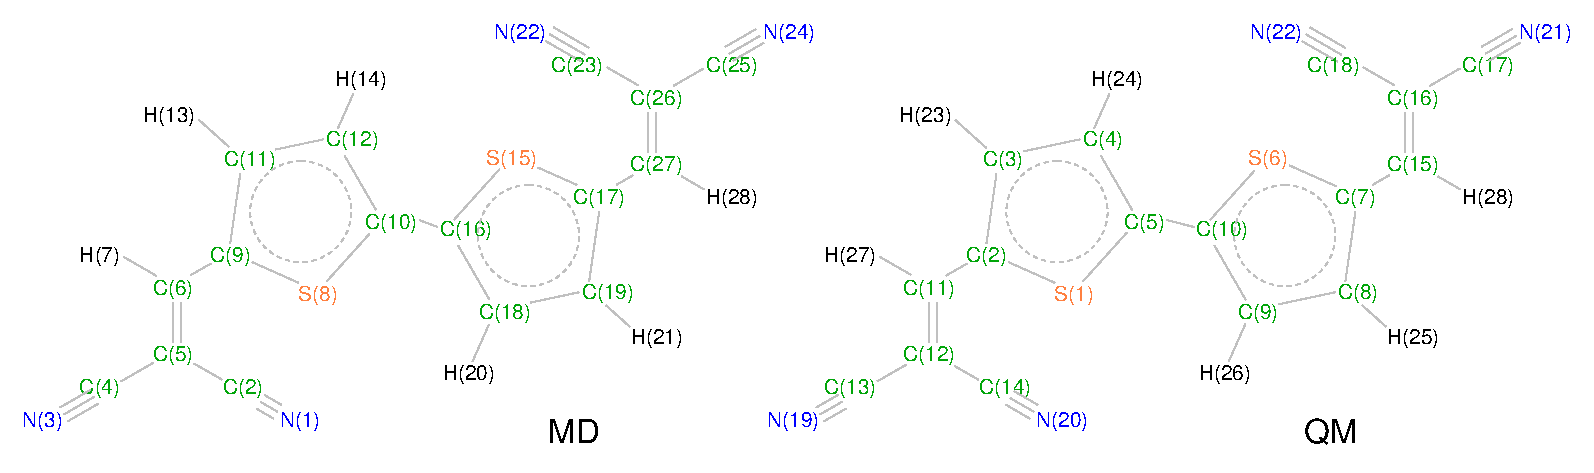
\includegraphics[width=\textwidth]{./fig/chemical_structure/dcv2t_gaussian} 
\caption{\small Atom order of \dcvt in the atomistic topology (MD) and qunatum chemical calculations (QM). The  link between two is established in the description of a conjugated segment shown in listing~\ref{list:conjugated_segments}.}
\label{fig:dcv2t_qm}
\end{figure}

\lstset{
  language=XML,
  frame=lines,
  basicstyle=\ttfamily\footnotesize,
  identifierstyle=\color{red},
  keywordstyle=\color{blue},
  showstringspaces=false,
  columns=fullflexible,
  commentstyle=\color{gray}\rmfamily\itshape,
  morekeywords={crgunit_type,ChargeUnitType,posname,orbname,basisset,transorb,reorg,nameneutr,namecrg,energy,beadconj,molname,name,monomer_atom_map,monomer_atom_weights},
}

\lstinputlisting[
 label=list:conjugated_segments, 
 caption={\small \xml file describing conjugated segments.
}]%
{./input/segments.xml}
\clearpage

%\noindent
%\suggestion{%
%crgunit\_type -> ConjugatedSegmentTypes \\ 
%ChargeUnitType -> ConjugatedSegmentType \\ 
%posname -> CoordinatesFile \\
%orbname -> OrbitalsFile \\
%transorb -> TransportOrbital \\
%reorg -> ReorganizationEnergy (do we need this here?) \\
%nameneutr -> ChargesNeutralFile \\
%namecrg -> ChargesChargedFile (do we need this here?) 
%}


